\documentclass{beamer}
\usepackage[utf8]{inputenc}
\usepackage{utopia}
\usetheme{Madrid}
\usecolortheme{default}
\title[About Beamer]
	{About Beamer in Presentation Making}
	\subtitle{A Short Story}
	\author[Author 1,Author 2]
	{Faculty 1\inst{1} \and Faculty 2\inst{2}}
	\institute{MIT,MAHE,Manipal}
	%
	\date[July-December 2019]{Dept of CSE,MIIT 2019}

	\logo{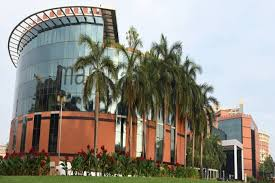
\includegraphics[height=2cm]{manipal2.jpg}}
	
	\AtBeginSection[]
	{
		\begin{frame}
		\frametitle{My Table of Contents}
		\tableofcontents
	\end{frame}
	
}


\begin{document}
\frame{\titlepage}
\begin{frame}
	\frametitle{Table of Contents}
	\tableofcontents
\end{frame}

\begin{frame}
	\frametitle{Sample for title}
		\begin{itemize}
		\item <1->Text of First Line \Pause
		\item <2->Text of Second Line \Pause
		\item <3->Text of Third Line \Pause
		\item <4->End of Overlays
		\end{itemize}
\end{frame}


\begin{frame}
	In this slide \Pause
	This text will be partially visible \Pause
	Now Everything 
\end{frame}

\begin{frame}
	\frametitle{Sample for title}
	\alert{highlighted} because it it important.
\end{frame}

\end{document}